
%\font\bfbig=cmbx10 scaled\magstep4  
%\font\bftitle=cmbx10 scaled\magstep1
%\font\smbftit=cmbx10 scaled\magstep2
%\font\amb=cmtt10 scaled\magstep0
%\font\bgtt=cmtt10 scaled\magstep1

% The "twoside" in documentstyle sets positioning of 
% page numbers on the page./
%   \documentstyle[fullpage,twoside]{report}
\documentclass{report}
\addtolength{\hoffset}{-15mm}
\addtolength{\textwidth}{3cm}
\addtolength{\textheight}{3.5cm}
\usepackage{makeidx,graphicx}
\makeindex

\begin{document}

\title{{\textbf{spsim}}
\vspace {1.0in}
{User Manual} \\ Version 1.0 (Alpha) }
\author {Filipe Maia}

\maketitle

\parindent=0pt 
\baselineskip=18pt 
\lineskip=0pt
\pagenumbering{roman}

\tableofcontents

\pagestyle{headings}

\def\delfo{$\delta_{fo}$~}
\def\delfc{$\delta_{fc}$~}
\def\qq{\qquad\qquad}
\def\hbar{\overline{h}}


% OFF WE GO .......

\chapter{Introduction} 
\label{intro}
\pagenumbering{arabic}

\vspace {0.1in}

spsim is a small program which aims to realistically simulate the output of a single
particle diffraction experiment.
The program reads it's input from a single file named spsim.conf which must reside
on the directory where the program is run.
It then runs for while and produces several VTK files related to the detector output
from the simualted an experiment.

\section{spsim.conf}
\label{tutorial}


spsim.conf is composed of several ``key = value lines;''.
All lines starting with ``\#'' are comments and not interpreted by the program.
{\em All values are in SI units!}

The required keys are:
\begin{itemize}
\item number\_of\_dimensions =  $<$int$>$ - currently only the value of 2 is valid. 
  Number of dimensions of the output.
\item input\_type = $<$string$>$ - currently only the value ``pdb'' is accepted. 
  Defines the type of the input structure on which the experiment is going to be performed.
\item pdb\_filename = $<$string$>$ - a string containing the path to the PDB file to be used.
\item detector\_distance = $<$float$>$ - the distance to the detector{\em in meters}.
\item detector\_width = $<$float$>$ - the width of the detector{\em in meters}.
\item detector\_height = $<$float$>$ - the height of the detector{\em in meters}.
\item detector\_pixel\_width = $<$float$>$ - the width of a single pixel{\em in meters}.
\item detector\_pixel\_height = $<$float$>$ - the height of a single pixel{\em in meters}.
\item detector\_quantum\_efficiency = $<$float$>$ - the quantum efficiency of the detector. 
  A number from [0.00,1.00] indicating 0 to 100\% efficiency
\item detector\_electron\_hole\_production\_energy = $<$float$>$ - energy required to produce an electron on the detector{\em in joules}.
\item detector\_readout\_noise = $<$float$>$ - RMS of the readout noise, in electrons per pixel.
\item detector\_dark\_current = $<$float$>$ - dark current of the CCD in electrons/(pixel.second).
\item detector\_linear\_full\_well = $<$float$>$ - maximum capacity of a pixel in electrons.
\item detector\_binning $<$int$>$ - number of pixels to bin. Binning is assumed to be the same in all dimensions
  so a value of 4 means 4x4 binning.
\item detector\_maximum\_value = $<$float$>$ maximum value that the detector output. For a 16 bit detector this would be $2^{16}$ or 65535.0.
\item experiment\_wavelength = $<$float$>$ the wavelength of the experiment {\em in meters}.
\item experiment\_exposure\_time = $<$float$>$ total exposure time in seconds.
\item experiment\_beam\_intensity = $<$float$>$ total beam intensity integrated over the entire exposure time in photons/$m^2$.
\end{itemize}

Due to the way libconfig works all floating point values {\em must} include 
a decimal point, otherwise they will be treated as 0. So for example
if your detector\_readout\_noise is 10 you need to write ``detector\_readout\_noise = 10.0;''.

Here is an example configuration file:

\begin{verbatim}
number_of_dimensions = 2;
input_type = "pdb";
pdb_filename = "DNA_triangle.pdb";
# 5cm detector distance
detector_distance = 5.000000e-02;
# 26.8mm x 26mm CCD
detector_width = 2.680000e-02;
detector_height = 2.600000e-02;
#20um square pixels 
detector_pixel_width = 2.000000e-05;
detector_pixel_height = 2.000000e-05;
# 15% quantum efficiency 
detector_quantum_efficiency = 1.500000e-01;
# 3.6 eV
detector_electron_hole_production_energy = 5.800000e-19;
detector_readout_noise = 1.000000e+01;
detector_dark_current = 1.000000e-01;
detector_linear_full_well = 2.000000e+05;
# 4x4 binning
detector_binning = 4;
detector_maximum_value = 65535.0;
#13 nm
experiment_wavelength = 1.300000e-08;
# 100fs
experiment_exposure_time = 1.000000e-13;
# 1e15 photons, 100um^2 area
experiment_beam_intensity = 1.0e25;
\end{verbatim}

\section{Output}
The output of spsim consists of the following files:

\begin{itemize}
\item spsim.confout - contains all information read by the program from spsim.conf
\item scattering\_factor.vtk - the scattering factors of the input molecule on the detector
\item thomson\_correction.vtk - the thomson correction factor for each pixel. Simply the differential electron cross-section times the pixel solid-angle
\item solid\_angle.vtk - the solid angle for each pixel
\item photon\_count.vtk - the number of photons detected by each pixel. This already takes into account the quantum efficiency and poisson noise.
\item electrons\_per\_pixel.vtk - electrons generated on each pixel due to the incomming photons.
\item real\_output.vtk - the value that detector output, including all the noise effects.
\item noiseless\_output.vtk - the value which the detector would output if there were no sources of noise.
\end{itemize}

An easy way to examine images is to use an excellent visualizer called VisIt produced by the LLNL
and freely available for many platforms. Please visit the page http://www.llnl.gov/visit/ for
more information, including installation details. From now on i'll assume that you have VisIt installed.
But any other VTK visualizer like should work.

\chapter{Theory}
The way spsim simulates the diffraction patterns is very simple. First it starts by calculating the reciprocal space coordinates
of the detector pixels, using the Ewald sphere construct ~\cite{Giacovazzo92}.
For each pixel $x,y$ on the detector at a distance $d$ from the source and at a wavelength $\lambda$ the reciprocal $h,k,l$ coordinates are:

\begin{figure}[!h]
\centering
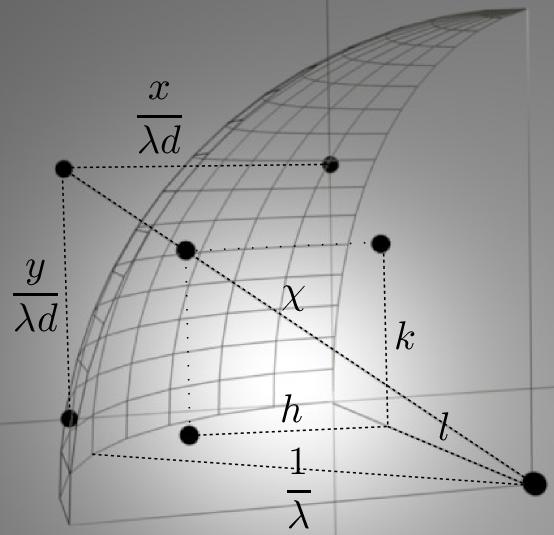
\includegraphics[scale=0.3]{ewald.png}
\label{ewald-construction}
\end{figure}


\begin{equation}
\chi = \sqrt{(\frac{x}{\lambda d})^2+(\frac{y}{\lambda d})^2+(\frac{1}{\lambda})^2}
\end{equation}
\begin{equation}
h(x,y) = \frac{x}{\lambda^2* d \chi}
\end{equation}
\begin{equation}
k(x,y) = \frac{y}{\lambda^2 d \chi}
\end{equation}
\begin{equation}
l(x,y) = \frac{1}{\lambda} - \frac{1}{\lambda^2\chi}
\end{equation}



Then the molecular scattering factors are calculated on those coordinates, using CCP4's atomsf.lib to get the atomic scattering factors.
Assuming $n$ atoms at positions $(x_j,y_j,z_j)$ and using $a_i$,$b_i$ and $c$ from atomsf.lib.
\begin{equation}
  f_{0j}(h,k,l) = \sum_{i=1}^{4} a_i exp(-b_i\Biggl[\frac{\sqrt{h^2+k^2+l^2}}{2}\Biggl]) + c
\end{equation}
\begin{equation}
  F(h,k,l) = \sum_{j=1}^{n} \{f_{0j}(h,k,l) \cos\{2 \pi (h x_j+k y_j + l z_j)\}\} + i \sum_{j=1}^{j=n}\{f_{0j}(h,k,l) \sin\{2 \pi (h x_j+k y_j + l z_j)\}\}
\end{equation}

After that the Thomson correction is applied. $K1$ and $K2$ are the relative vertical and horizontal polarized parts of the beam.
That an horizontal scaterring plane $K1 = 0$ and $K2 = 1$ and vice versa. For unpolarized light $K1 = K2 = 0.5$.
$P$ is the polarization factor. $2\theta$ is the angle between the primary beam and the direction of observation.
$I_{eTh}$ is the density of the scattered radiation, $I_i$ is the intensity of the indicent radiation,
$e$ is the charge of the electron, $m$ the mass of the electron and $c$ the speed of light.
$\frac{e^2}{mc^2}$ is known as the classic electron radius.


\begin{equation}
   P(\theta) = K_1 +K_2 \cos^2(2\theta)
\end{equation}
\begin{equation}
   \frac{I_{eTh}}{I_i} = \frac{e^4}{m^2c^4} \times P(\theta) = Thomson(\theta)
\end{equation}

The Thomson correction is applied to each pixel according to it's solid angle, and then the total number of photons that arrive to each pixel is calculated.
$\Omega$ is the solid angle and $A_{px}$ is the pixel area projected on a plane passing through the center of the pixel and normal to the direction of observation.


\begin{equation}
   \Omega(x,y) = \frac{A_{px}}{x^2+y^2+d^2}
\end{equation}

The number of photons that arrive at each pixel, $Ph_{inc}$ is then given by:


\begin{equation}
   Ph_{inc}(x,y) = Thomson(\theta) \times \Omega(x,y) \times F(hkl(x,y)) \times I_i
\end{equation}

From those pixel that arrive at each pixel only a certain number is detected. The percentage that on average is detected is known as
{\em quantum efficiency}($\tau$) and is wavelength dependent. $Poisson(x)$ returns a poisson distributed number with mean $x$.
The number of photons detected on each pixel($Ph_{det}$) is then:


\begin{equation}
  Ph_{det}(x,y) = Poisson(Ph_{inc}(x,y) \times \tau)
\end{equation}

Using $\mu$ to represent the energy to produce one electron hole, the number of electrons generated on the pixel by the detected photons($el_{gen}$ is then simply:


\begin{equation}
  el_{gen}(x,y) = \frac{Ph_{det}(x,y) \times \frac{hc}{\lambda}}{\mu}
\end{equation}


Representing the maximum value output by the detector by $V_{max}$, the binned pixels by $px_{bin}$, the pixel linear full well by $W_{max}$ exposure time by $t$
dark current by $\iota$ and readout noise by $N$,
 the final output is then calculated by:


\begin{equation}
  Output(x,y) = \sum_{x_{bin},y_{bin}}^{px_{bin}} \{\left( el_{gen}(x_{bin},y_{bin}) + \iota t \right)\}  + Gaussian(N) \times \frac{V_{max}}{W_{max}}
\end{equation}

Where Gaussian(x) returns a normally distributed random number with mean 0 and standard deviation x.

The noiseless output is then calculated by:

\begin{equation}
  Noiseless(x,y) = \sum_{x_{bin},y_{bin}}^{px_{bin}} \frac{Ph_{inc}(x_{bin},y_{bin}) \times \tau \times  \frac{hc}{\lambda}}{\mu} \times \frac{V_{max}}{W_{max}}
\end{equation}


\chapter{Installation }

spsim should compile in any linux distribution and most kinds of Unix. It might also compile in windows under cygwin although that
has not been tested.


To install first simply extract the source code, go to the libconfig-0.9 directory inside of the source code directory, run configure followed by make,
move to the previous directory and run make. For example:

\qq {\tt  \$ tar -zxvf spsim-1.0.tar.gz}

\qq {\tt  \$ cd spsim-1.0}

\qq {\tt  \$ cd libconfig-0.9}

\qq {\tt  \$ ./configure}

\qq {\tt  \$ make}

\qq {\tt  \$ cd ..}

\qq {\tt  \$ make}

You now should have a binary called ``spsim'' in your ``spsim-1.0'' directory, ready to run.


If you wish to turn off MPI support you need to edit the Makefile on the ``spsim-1.0'' directory and change the MPI = ON line
to MPI = OFF.


\vspace {4.0 in}

You can now run the examples by going to the examples directory and running spsim:

\qq {\tt  \$ cd examples}

\qq {\tt  \$ ../spsim}

This should produce several files including ``real\_output.vtk'' and ``noiseless\_output.vtk'' that you can now take a look at.
They should look like this:

\begin{figure}[!h]
\centering
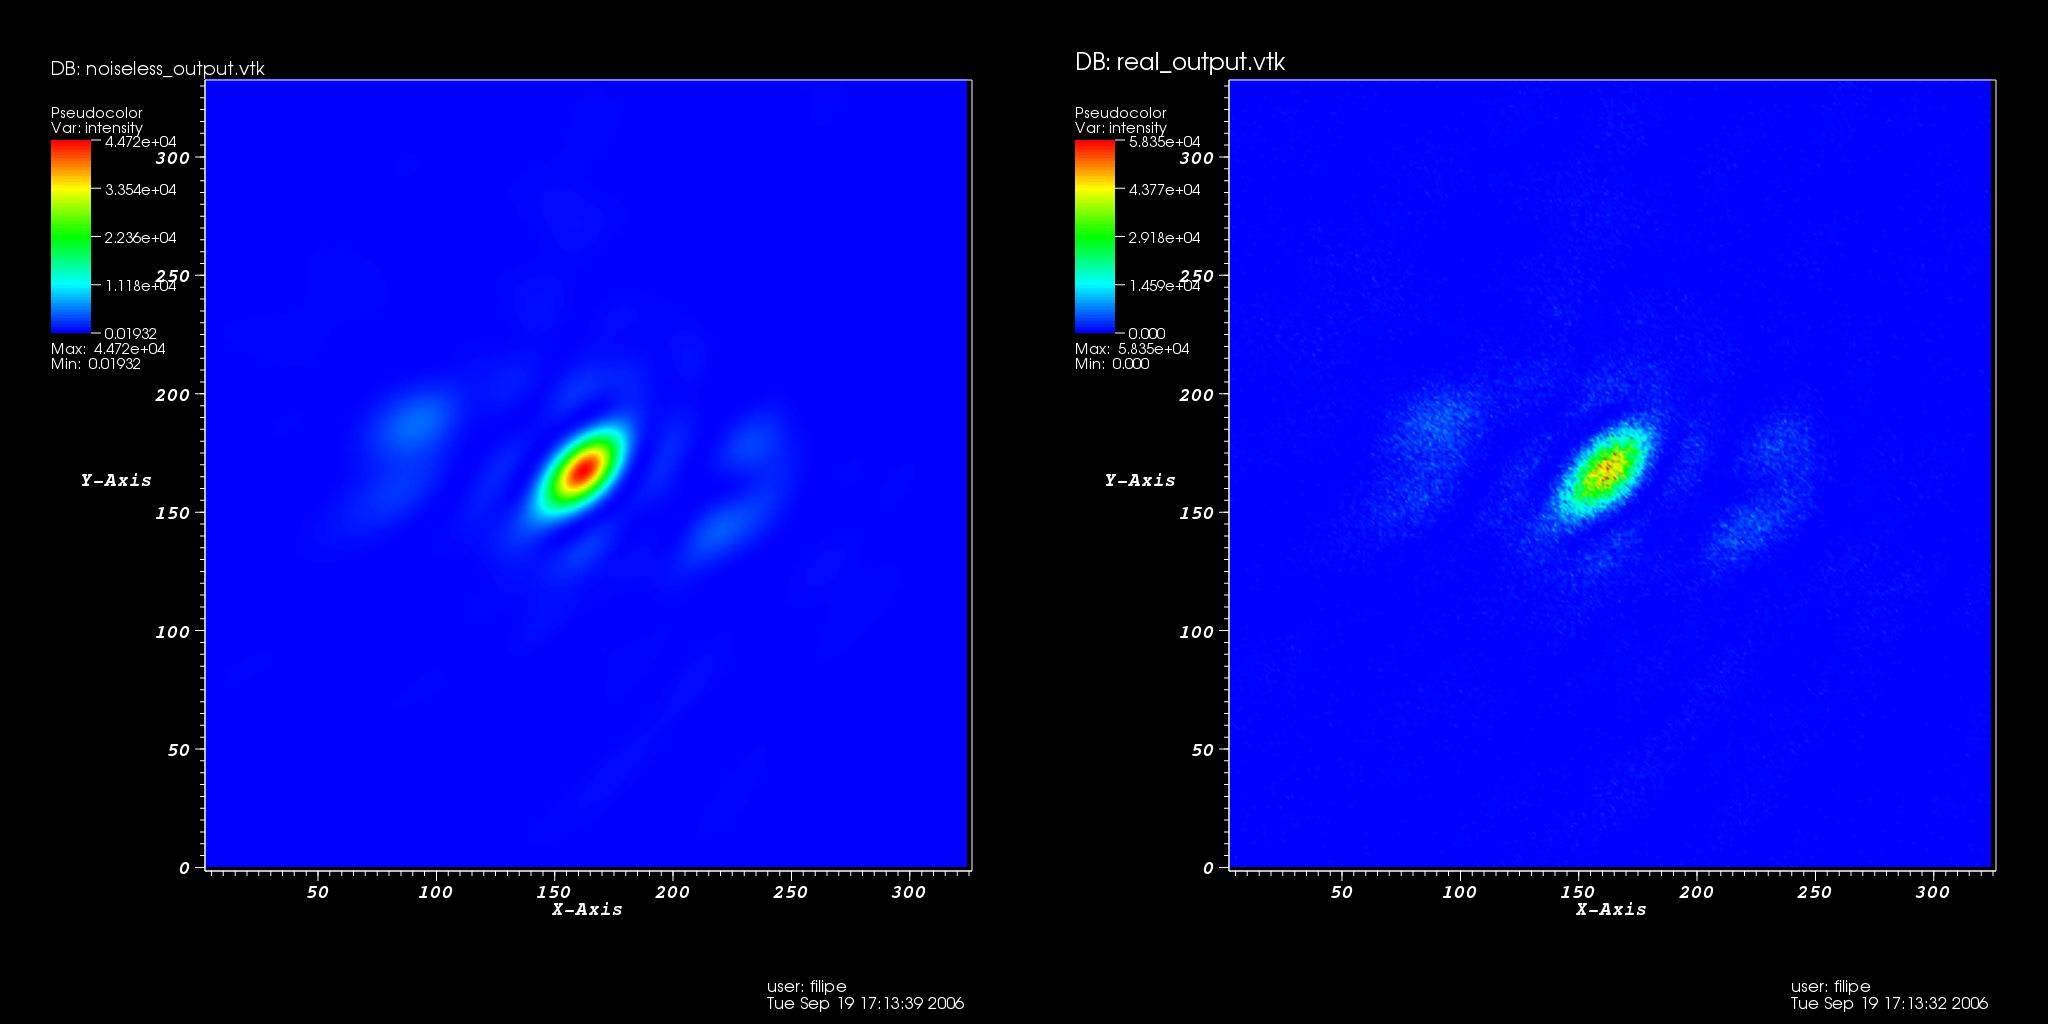
\includegraphics[scale=0.2]{example.png}
\label{ewald-construction}
\end{figure}

Congratulations you have successfully installed spsim!


\bibliographystyle{acm}
\bibliography{imaging}

\end{document}
 